\documentclass{beamer}
\usepackage{tcolorbox}
\usepackage{hyperref}
\usepackage{../notation}

%\beamerdefaultoverlayspecification{<+->}
% \newcommand{\data}{\mathcal{D}}
% \newcommand\Item[1][]{%
% 	\ifx\relax#1\relax  \item \else \item[#1] \fi
% 	\abovedisplayskip=0pt\abovedisplayshortskip=0pt~\vspace*{-\baselineskip}}

\graphicspath{ {imgs/} }

\usetheme{metropolis}           % Use metropolis theme


\title{Gradient Descent vs Stochastic Gradient Descent}
\date{\today}
\author{Nipun Batra}
\institute{IIT Gandhinagar}
\begin{document}
	\maketitle

	\begin{frame}{}
\begin{columns}
  \begin{column}{0.5\textwidth}{\underline{Gradient Descent}}
    \begin{itemize}
        \item Slower in speed\\ (Needs to see many examples before update)
	\item Smooth convergence
	\item $epochs = iterations$
    \end{itemize}
	\vspace{0.5cm}
	\centering
	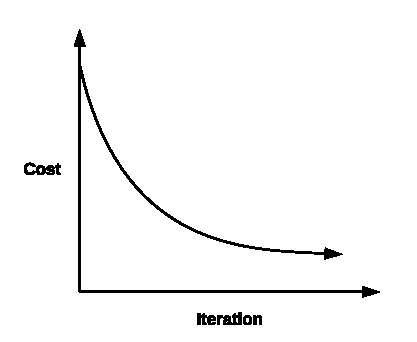
\includegraphics[width = 0.8\textwidth]{gd-cost-iter-curve}
  \end{column}

  \begin{column}{0.5\textwidth}{\underline{Stochastic Gradient Descent}}
     \begin{itemize}
        \item Faster in speed
	\vspace{0.5cm}
	\item Noisy convergence
	\item $epochs = \dfrac{iterations}{examples}$
     \end{itemize}
	\vspace{0.5cm}
	\centering
	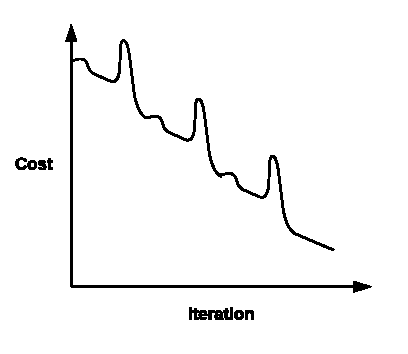
\includegraphics[width = 0.8\textwidth]{sgd-cost-iter-curve}
  \end{column}
\end{columns}
	\end{frame}
	


\end{document}